\section{What lives in the repository?}
%
%As we have presented before git keeps snapshots of how your system
%looked like on a certain moment in time. This moment in time is
%represented in git by a commit. A commit points to a tree, that
%represents the structure of your system on that moment. So a tree
%contains others trees and/or blobs. In git the files are not kept. 
%What git keeps is a blob that represents the content of files. The
%relation between the path of a file and the content of that path 
%is kept on the trees corresponding to that path. \par
%
%\subsection{Objects}
%All objects are identified by an hash 
%defined by their contents. Thus, when two files have the same
%content, they will have the same identification. \par
%
%There are the following types of objects in the world of Git:
%
%\begin{itemize}
%\item A Blob that stores file data and can be seen as a file
%\item A Tree that stores blobs and other trees, thus can be seen as folders.
%\item A Commit that points to a snapshot of the repository at a given moment.
%Also points to previous commit(s) and identifies the user that made the commit.
%\item A Tag points to special commits. For example, a commit that has the beta
%version of some program.
%\end{itemize}
%
%\begin{figure}[h!] 
%	\caption{A commit object pointing to a tree}
%	\centering
%	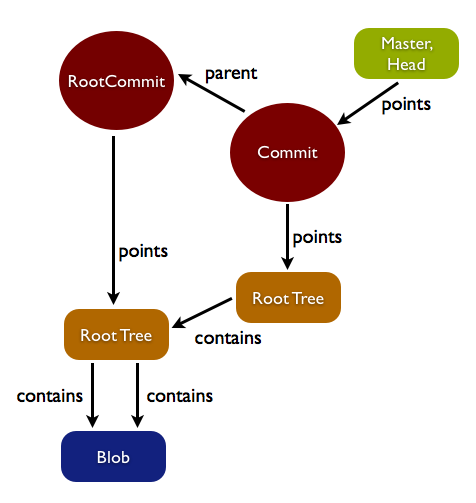
\includegraphics[scale=0.50]{images/commitobject.png}
%\end{figure}

%\subsection{Branches}
%One of the trump cards of Git it's his definition of branches. Other VCS
%have a copy of the entire repository for each branch made. Thus, branches
%operations in those VCS are slow and hard to use. Now Git, just uses 
%pointers for branches. In fact, when creating a new branch the only thing
%done is the creation of new pointer that will point to the current commit. \par
%So, the branches operations in Git turn to be fast and easy to use. \par
%It's important to say that exists a special pointer called "Head" that will 
%always point to the current commit. \par

